\documentclass[notitlepage]{article}
\usepackage[left=1in, right=1in, top=1in, bottom=1in]{geometry}

\usepackage{titling}

\pretitle{\begin{center}\Huge\bfseries}
\posttitle{\par\end{center}\vskip 0.5em}
\preauthor{\begin{center}\Large\ttfamily}
\postauthor{\end{center}}
\predate{\par\large\centering}
\postdate{\par}

% Bibliography
\usepackage[backend=bibtex, style=numeric]{biblatex}
\addbibresource{references.bib}

% Graphics
\usepackage{graphicx}
\usepackage{tikz-cd}

% Math
\usepackage{amsfonts} % mathbb
\usepackage{amsmath} % amsmath

% Align two equations
\usepackage{multicol}

% Code listings
\usepackage{listings}

\title{Tactic and (co)algebraic reasoning}
\author{Rodrigo Raya\\[0.5cm]{Advisor: Prof. Viktor Kunc\v ak} \\ [0.5cm]{Laboratory for Automated Reasoning and Analysis (LARA) \\ [0.5cm]}}
\date{\today}
\begin{document}

\maketitle
\thispagestyle{empty}

\begin{abstract}
The purpose of this report is to introduce tactical reasoning and the theory of (co)algebras in the design of the Isabelle proof assistant. In a previous presentation, I studied how tactical reasoning was introduced by Milner in the LCF system. In this work, I study how tactical reasoning is achieved in one of LCF's descendants. Two particular tactics were developed in the context of mathematical theorem proving. Furthermore, I describe the general theory of (co)algebras and report on its use in Isabelle to provide a solid foundation for its (co)datatype package. Further research is needed to compare this approach to other systems that reduce the study of coalgebras to algebras and discuss the advantages and disadvantages of both approaches.
\end{abstract}

\section{Tactical reasoning}

In \cite{milner1984use}, Milner discussed the introduction of tactics and tacticals. He implemented these features in the Edinburgh LCF proof assistant. LCF, the mechanization of Scott’s Logic of Computable Functions, was probably the first theoretically based yet practical tool for machine assisted proof construction and was quoted as one of the reasons why Milner received the Turing Award in 1991. A summary of this work can be seen in \cite{presentation}. 

Modern proof assistants such as Isabelle provide users with a large collection of specialized tactics to facilitate the theorem proving process. These tactics come in three different levels of abstraction. Users are normally presented the Isar language \cite{wenzel2002isabelle}. This language permits modular reasoning similar to that found in normal high-level proofs. The underlying implementation uses a metalanguage written in ML that encodes the logic and the transformations allowed on it. This is the level in which Milner developed his theory of tactics and our study goal in this semester project. Finally, the Eisbach language was developed to provide users with a high-level language to design new proof methods by reusing the predefined ones. 

Figure \ref{fig:isar} gives the high-level representation of Isar proof processing in contraposition with the usual state of things in tactical theorem proving. The richness of Isar language greatly facilitates the proving process. However, I illustrate in this section some examples in which the user might need to resort to specialized tactics, forcing us to descend to the metalanguage of the system. 

\begin{figure}
	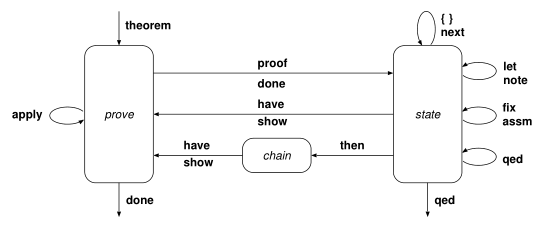
\includegraphics[scale=0.65]{img/isar.png} 
	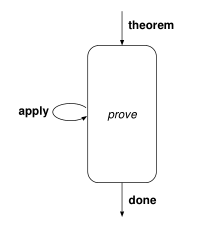
\includegraphics[scale=0.65]{img/tactics.png}
	\caption{Transitions of Isar proof processing and tactical theorem proving (taken from \cite{wenzel2002isabelle})}
	\label{fig:isar}
\end{figure}

I give first some background references that may help during the process of learning to program in Isabelle/ML. The Isabelle/Isar Implementation manual comes with the distribution and provides a detailed overview of the Isabelle/ML level. I would recommend \cite{wenzel2002isabelle} for the foundations of the system. For a practical introduction to program Isabelle/ML is the Isabelle Cookbook \cite{cookbook}. I focused on the study of on tactical reasoning. However, the sections teaching how to create new proof commands, parsing specifications and writing new definitional packages helped me in understanding what is the connection between Isabelle/Isar and Isabelle/ML. A fresh perspective of the system can be found on \cite{wolff2019my}.

\subsection{An associativity proof}

I recently finished a proof of the group law for elliptic curves on Edwards form \cite{Gauss_Sums-AFP}. The hardest part on this classical exercise in theorem proving is showing that the group law is associative. In my setting, this amounts in showing that the following equation holds:

\[
(p_1 \oplus_i p_2) \oplus_j p_3 = p_1 \oplus_k (p_2 \oplus_l p_3)
\]

Here $i,j,k,l \in \{0,1\}$ and $\oplus_0,\oplus_1$ are well-defined operations on elliptic curves points. After completing the proof I found that the different proofs were actually very similar. The proof can be found in \cite{associativity}. In essence, we abstract the different 16 proofs into a single function yielding for each parameter combination the corresponding theorem. The theorem to be proven as well as the method of proving it is a function of the input parameters. This process can be observed in function \textit{concrete\_assoc}.

To the side, I also investigated the design of the rewrite tactic. This method supersedes the substitution tactic which needs to specify the position of the subterm to which we apply certain rule. In \cite{noschinskipattern}, the authors explain the design of a language to specify subterms to be rewritten with a pattern-matching approach. Internally, the implementation added commands \textit{in} (selecting of subterms of a term) and \textit{concl} (selecting the conclusion of the goal as the target term) to our apply-style commands. However, I only found this out when debugging the ML implementation for the rewriting library. This leads me to the last remark of this section.

Some tips on how to debug ML source code may be appreciated for future users. In \cite{explore}, it is explained how to edit theories that are read-only by default. In \cite{navigate}, it is explained how to browse ML files. For limited debugging support of ML code, see chapter 5 of the JEdit manual.

This section provides a good example for the section on structured proofs in the Isabelle Cookbook. 

\subsection{Rewriting sines}

I present a small tactic illustrating some common idioms for Isabelle/ML. The idea is to rewrite sine expressions whose arguments contain sums of multiples of $\pi$. I chose to encode this as a \textit{simproc}. These simprocs are special rewriting procedures called by the simplifier to solve theory-specific goals. Other examples, like a tactic to facilitate the application of Taylor theorem contribute to bridge the gap between mathematicians expectations and theorem proving tools. 

The high-level idea of the tactic \cite{sines} is as follows:

\begin{enumerate}
\item Define a function SIN\_SIMPROC\_ATOM x n = x + of\_int n * pi.
\item Write a conversion sin\_atom\_conv that rewrites of\_int n * pi to SIN\_SIMPROC\_ATOM 0 n and everything else into SIN\_SIMPROC\_ATOM x 0. 
\item Write a conversion that descends through +, applies sin\_atom\_conv to every atom, and then applies some kind of combination rule like:

 SIN\_SIMPROC\_ATOM x1 n1 + SIN\_SIMPROC\_ATOM x2 n2 = \\
 SIN\_SIMPROC\_ATOM (x1 + x2) (n1 + n2).
\item In the end, I have rewritten the original term to the form sin (SIN\_SIMPROC\_ATOM x n), and then I apply some suitable rule to that.
\end{enumerate}

A conversion is essentially a function of type cterm $\to$ thm which takes a cterm ct and returns a theorem of the form ct $\equiv$ …, i.e. it's a form of deterministic rewriting (a conversion can also fail by throwing a CTERM exception, by convention). There are a lot of combinators for building and using these in Pure/conv.ML

The resulting theorem is then provided to the user transparently, since the simproc is activated by the simplifier. The details of the implementation can be seen in \cite{sineimplementation}.

\section{(Co)algebras}

I also tried to answer the question: what is an algebraic datatype? I studied the answer to this question from the point of view of category theory \cite{barr1990category}. This theory models (co)datatypes and (co)induction through the concept of coalgebras \cite{smyth1982category} \cite{denecke2009universal} \cite{rutten}. It is somewhat surprising that these concepts have found their way into the implementation of proof assistants \cite{traytel} \cite{blanchette2014cardinals}. There seem to be problems with other implementations reducing coinduction to induction \cite{blanchette2015foundational} \cite{coq1} \cite{coq2} \cite{coq3}. 

\subsection{Theoretical background}

Let $F: Set \to Set$ be a functor. An $F$-algebra is given by a set $A$ and a mapping $\alpha: F(A) \to A$. $\alpha$ is called the structure mapping of the $F$-algebra. A $F$-homomorphism $f$ between two F-algebras $(A,\alpha),(B,\beta)$ is a mapping that makes the following diagram commutative:

\begin{tikzcd}
F(A) \arrow[d, "\alpha"] \arrow[r, "F(f)"] & F(B) \arrow[d, "\beta"] \\
A \arrow[r, "f"] & B 
\end{tikzcd}

One can form a category $Set^F$ whose objects are all $F$-algebras and its morphisms are the families of $F$-homomorphisms. Given an $F$-algebra $\mathcal{A} = (A,s)$, a subalgebra of $\mathcal{A}$ is given by a $S \subseteq A$ together with a morphism $\beta_S:F(S) \to S$ such that the inclusion $i: S \to A$ is an homomorphism. The notions of coalgebra, coalgebra homomorphism, category $Set_F$ of all coalgebras and subcoalgebra are obtained reversing the arrows in the above definitions. 

An initial $F$-algebra is an initial object in $Set^F$. A terminal $F$-coalgebra is a terminal object in $Set_F$. As a consequence, if any of these exist, it is unique up to isomorphism. A classical result by Lambeck states that the structure mapping of an initial algebra (dually, a final coalgebra) is an isomorphism. As a consequence, the powerset functor $\mathcal{P}: Set \to Set$ cannot have initial or final coalgebras since their existence would contradict Cantor's theorem. 
	
A relation $R \subseteq S \times T$ is an $F$-congruence if there exists an $F$-algebra structure $(R,\gamma)$ such that the projections $\pi_i$ are $F$-homomorphisms:
	
\begin{tikzcd}
F(S) \arrow[d, "\alpha"] & F(R) \arrow[l, "F(\pi_1)",swap] \arrow[d, "\gamma",dashed] \arrow[r, "F(\pi_2)"] & F(T) \arrow[d, "\beta"]\\
S  & R \arrow[l, "\pi_1"] \arrow[r, "\pi_2",swap] &  T
\end{tikzcd}

dually, one gets the notion of $F$-bisimulation. If one defines the diagonal of a set $A$, as the set: \[\Delta(A) = \{(a,a). a \in A\}\] one can state the (co)induction principles as follows:

\begin{itemize}
	\item Induction: every congruence relation on an initial algebra contains the diagonal.
	\item Coinduction: every bisimulation relation on a final coalgebra contains the diagonal.
\end{itemize}

it is straight-forward to reduce the traditional induction principle on natural numbers, coinduction principle on streams or the view on (co)induction as least (greatest) fixed points of $F$ to the above principles.

\subsection{Functional programming and (co)algebras}

Let $A_1, \ldots , A_k$ be sets and $n_1, \ldots n_k \in \mathbb{N}$. $F$ is polynomial if it is of the form: \[F(X) = A_1 \times X^{n_1} + \ldots + A_k \times X^{n_k}\] where $\times$ is the cartesian product and $+$ is the disjoint union of sets. In this categorical view, a datatype is the initial algebra and a codatatype is the final coalgebra of a polynomial functor. If $(T,c)$ is an initial algebra (final coalgebra) for $F$, one can write: \[c: A_1 \times T^{n_1} + \ldots + A_k \times T^{n_k} \to T\] and decompose $c = [c_1,\ldots,c_k]$ as: \[c_i: A_i \times T^{n_i} \to T\] Since $+$ stands for the disjoint union of sets. By Lambek's lemma, $T$ is completely determined by the $c_i$. 

In a programming language, the corresponding constructs are written as follows:


\noindent\begin{minipage}{.5\linewidth}
\begin{align*}
\text{datatype} \; T &= c_1 \; of \; A_1 \times T^{n_1} \\
&\;\;\vdots \notag \\
&| = c_k \; of \; A_k \times T^{n_k} \\
\end{align*}
\end{minipage}%
\begin{minipage}{.5\linewidth}
\begin{align*}
\text{codatatype} \; T &= c_1 \; of \; A_1 \times T^{n_1} \\
&\;\;\vdots \notag \\
&| = c_k \; of \; A_k \times T^{n_k} \\
\end{align*}
\end{minipage}

Geuvers \cite{geuvers2007iteration} gives a clear account on how iteration, primitive recursion and case analysis can be understood categorically. For instance, checking initiality of datatypes leads to definitions by iteration. To see an example, consider the natural numbers $\mathbb{N}$ as an algebra over the functor $F(X) = 1 + X, F(f) = id + f$ where $1 = \{*\}$ and $*$ is a non-natural number. The structure map we consider is $[zero,succ]$ where $zero$ assigns $*$ to $1$ and $succ$ assigns each natural number to its successor. We show that there exists a unique $f$ such that the following diagram commutes:
	
\begin{tikzcd}
1 + \mathbb{N} \arrow[r, "F(f)"] \arrow[swap]{d}{[zero,succ]} & 1+X \arrow[d, "\alpha"] \\
\mathbb{N} \arrow[r, "\exists ! f",swap,dashed] & X
\end{tikzcd}
	
That is, $\alpha \circ N(f) = f \circ [zero,succ]$ or equivalently $f(0) = \alpha(*)$ and $\forall x \in \mathbb{N}. f(x+1) = \alpha(f(x))$. By natural induction, there is a unique $f$ satisfying this definition.	Since $f$ is defined iterating over $\alpha$, it is sometimes denoted $iter(\alpha)$. More generally, we can see our initial algebra endowed with an iterator mapping $iter$ sending each $\alpha$ to the function $f$ it defines. 

Primitive recursion on natural numbers can be encoded with the following scheme:

\begin{itemize}
\item $h(0) = g_1(*)$
\item $h(succ(n)) = g_2(h(n), n)$ 
\end{itemize}

If $g: 1 + B \times \mathbb{N} \to B$ is given, the above definition corresponds to the existence of a unique mapping $h$ making the following diagram commutative:

\begin{tikzcd}
1 + \mathbb{N} \arrow[swap]{d}{[zero,succ]} \arrow[dashed]{r}{F \langle h,id \rangle} & 1 + B \times \mathbb{N} \arrow[d,"g"] \\
\mathbb{N} \arrow[r, "\exists ! h",swap, dashed] & B
\end{tikzcd}

In general, $h = \pi_1 \circ iter\langle g, in \circ F(\pi_2)\rangle$. Since $h$ is defined recurring to $g$, we write it $h = rec(g)$ and for any initial algebra we can establish a mapping $rec$ assigning to each extra parameter supplier $g$, the function $h$ it defines.

Finally case analysis on natural numbers corresponds to the following scheme:

\begin{itemize}
	\item $h(0) = g_1(*)$
	\item $h(succ(n)) = g_2(n)$
\end{itemize}

If $g: 1 + \mathbb{N} \to B$ is given, the above definition corresponds to the existence of a unique mapping $h$ making the following diagram commutative:

\begin{tikzcd}
1 + \mathbb{N} \arrow[swap]{d}{[zero,succ]} \arrow{dr}{g}  \\
\mathbb{N} \arrow[r,"\exists ! h",dashed,swap] & B
\end{tikzcd}

Coiteration, corecursion and cocase analysis are encoded as the dual of the above notions.

\subsection{Building initial and final (co)algebras}

In this section, I state some theorems that guarantee the existence of usual (co)datatypes. The first result is due to Adámek and Barr and can be seen as a generalization of Kleene's fixed-point theorem:

\begin{itemize}
	\item Let $\mathcal{C}$ be a category with initial object $0$ and colimits for any $\omega$-chain. If $F: \mathcal{C} \to \mathcal{C}$ preserves the colimit of the initial $\omega$-chain, then the initial $F$-algebra is $\mu(F) = \text{colim}_{n < \omega} F^n 0$.
	\item Let $\mathcal{C}$ be a category with terminal object $1$ and limits for any $\omega^{op}$-chain. If $F: \mathcal{C} \to \mathcal{C}$ preserves the limit of the terminal $\omega^{op}$-chain, then the terminal $F$-coalgebra is $\nu(F) = \text{lim}_{n < \omega^{op}} F^n 1$.
\end{itemize}

As a consequence, we have:

\begin{itemize}
	\item Any polynomial functor on $Set$ admits an initial algebra and a final coalgebra.
\end{itemize}

For the construction in Isabelle, there are two points to be made. First, the above theorems do not apply to all the functors of interest for Isabelle theories. Some examples that are not dealt with include: the finite powerset ('a fset), countable powerset ('a cset), finite multisets ('a multiset) and the discrete probability distributions ('a pmf). As an example, finite depth finitely branching trees can be defined with this functor:

\begin{lstlisting}
datatype 'a tree = Node 'a ('a tree fset)
\end{lstlisting}

Instead, the notion of bounded endofunctor is introduced, see section 4.6 of \cite{jacobs2005introduction}. As remarked there both approaches seem to be related by transfinite induction. A second point to be made is that the above construction is not enough even for the simple polynomial functors that constituted our (co)datatypes. This is because arbitrary limits require reasoning about infinite type families, which goes beyond HOL capabilities.

\subsection{The Isabelle approach}

In a real proof assistant, the user specifies some type constructors, such as:

\begin{lstlisting}
'a List = Nil | Cons 'a ('a List) 
\end{lstlisting}

which can be understood as a fixed point equation $X = 1 + A \times X$ on types. The Isabelle's (co)induction package has to derive appropriate theorems for such an equation. Given such a user definition, how do we derive the corresponding functorial structure? Given the functorial structure, how do we derive in the logic the (co)induction principles, introduction rules and (co)case analysis? This study can be found on \cite{traytel} and the practical implementation in \cite{boundednat} which shows in apply-style the rewriting steps performed by the definitional package. 


\subsubsection{Functorial structure}

HOL can be modeled as a category using the universe of types $U$ as objects and functions between types as morphisms. A type constructor $(\alpha_1,\ldots,\alpha_n)F$ together with a mapping: \[\text{Fmap}: \overline{\alpha} \to \overline{\beta} \to \overline{\alpha} F \to \overline{\beta} F\] such that $\text{Fmap} \; \text{id} = \text{id}$ and $\text{Fmap} (\overline{g} \circ \overline{f}) = \text{Fmap} \, \overline{g} \circ \text{Fmap} \, \overline{f}$ gives the notion of functor $(\text{F}, \text{Fmap})$ whose action on objects is $\text{F}$ and on morphisms is $\text{Fmap}$. In order to formalize initial and final (co)algebras, the notion of functor is enriched into the notion of bounded natural functor. An n-ary bounded natural functor is a tuple $($F, Fmap, Fset, Fbd$)$ where:

\begin{itemize}
	\item $F$ is an n-ary type constructor.
	\item $\text{Fmap}: \overline{\alpha} \to \overline{\beta} \to \overline{\alpha} F \to \overline{\beta} F$
	\item $\forall i \in \{1,\ldots,n\}.$ Fset$_i: \overline{\alpha}F \to \alpha_i \text{ set}$
	\item Fbd is an infinite cardinal number.
\end{itemize}

satisfying the following:

\begin{itemize}
	\item (F,Fmap) is a binary functor.
	\item Fset$_i: \overline{\alpha}F \to \alpha_i \text{ set}$ is a natural transformation from:
	
	$((\alpha_1,\ldots,\alpha_{i-1},\textunderscore,\alpha_{i+1},\ldots,\alpha_n)F, \text{Fmap})$ to $(\text{set}, \text{image})$.
	\item (F,Fmap) preserves weak pullbacks.
	\item $\forall a \in \text{Fset}_i \, x,  i \in \{1,\ldots,n\}. f_i \, a = g_i \, a \implies \text{Fmap} \, \overline{f} \, x = \text{Fmap} \, \overline{g} \, x$
	\item The following cardinal bound conditions hold:
	
	$\forall x : \overline{\alpha} F, i \in {1,\ldots,n}. |\text{Fset}_i \, x | \le \text{Fbd}$
\end{itemize}

There is a key observation to this definition. The authors call it the \textit{shape and content} intuition. Indeed, if one writes the definition of natural transformation for the second axiom for the inclusion mapping $f = i$, one obtains that $\text{Fmap} \, i = i$. So inclusion lifts to the inclusion. Thus, the notion of subalgebra is greatly simplified in this context. If $(A,t)$ is a $F$-subalgebra of the algebra $(B,s)$, then the inclusion $i: A \to B$ is an $F$-algebra homomorphism and $\text{Fmap} \, i = i$ so the subalgebra equation simplifies to $s \circ i = i \circ t$ which implies that $t = s|_{F(A)}$. Thus, for a BNF, a subalgebra can be given by a subset together with a particular restriction of the structure mapping.

\subsubsection{Induction principle}

In this section, I describe the construction of the initial algebra in Isabelle/HOL. The derived induction principles can be seen in \cite{traytel}. The construction happens in two stages: first we build a weakly initial algebra and then the initial algebra is built from the former. The authors present the second step with a construction \textit{from above} of the minimal algebra generated by $\emptyset$, but in practice, they implement a construction \textit{from below} that is less intuitive since it uses transfinite induction. Here, I describe the abstract construction which benefits from the remarks made in the previous section on the characterization of subalgebras for bounded natural functors.

Let $\mathcal{A}=(A,s)$ be an $F$-algebra. Set $M_s = \bigcap_{B. (B,s) \text{is a subalgebra of (A,s)}} B$ then: \[\mathcal{M}(\mathcal{A}) = \Big(M_s,s \Big|_{M_s} \Big)\] is the $F$-subalgebra generated by $\emptyset$. We call it the minimal algebra generated by $\mathcal{A}$. $\mathcal{M}(\mathcal{A})$ is said to be the subalgebra generated by $\emptyset$ in the sense that it is the intersection of all subalgebras containing $\emptyset$.

There exists at most one morphism from $\mathcal{M}(\mathcal{A})$ to any other $F$-algebra $(Y,t)$ (*). Since, if $f,g$ are two such morphisms, we can show that: $$B = \mathcal{M}(\mathcal{A}) \cap \{x \in \mathcal{A}. f(x) _= g(x)\}$$ is a $F$-subalgebra of $\mathcal{A}=(A,s)$. Indeed, by our remarks, it suffices to note that $M_s \cap \{x \in \mathcal{A}. f(x) _= g(x)\} \subseteq M_s$ and consider the structure map $s|_B$. This leads to a subalgebra of $\mathcal{M}(\mathcal{A})$ which can be naturally seen as a subalgebra of $\mathcal{A}$. By definition of $\mathcal{M}(\mathcal{A})$, $M_s \supseteq B$ and thus $\forall x \in M_s. f(x) = g(x)$. Thus, the morphisms are equal. We will use this observation in what follows.

Here is the naive approach to the construction of an initial $F$-algebra.

\begin{enumerate}
	\item Set $\mathcal{R} = \prod \{\mathcal{A}. \mathcal{A} \text{ is an algebra}\}$.
	\item Given an algebra $\mathcal{A}$, note $h$ the projection morphism from $\mathcal{R}$ to $\mathcal{A}$.
	\item Then $h|_{\mathcal{M}(\mathcal{R})}$ is the unique morphism between $\mathcal{M}(\mathcal{R})$ and $\mathcal{A}$.
	\item Since the construction does not depend on the chosen algebra $\mathcal{A}$,  $\mathcal{M}(\mathcal{R})$ is the desired initial algebra.
\end{enumerate}

The naive approach cannot be encoded in HOL. First, one cannot quantify over infinite type collections. Second, the product of the carrier sets of all algebras, fails itself to be a set. Instead, we split the construction in two phases:

\begin{enumerate}
	\item Given an $F$-algebra $\mathcal{A}$ we know that there exists at most one morphism $\mathcal{M}(\mathcal{A}) \to \mathcal{A}$. But from our remarks above, for bounded natural functors, the inclusion is one such morphism. So there is exactly one morphism $g: \mathcal{M}(\mathcal{A}) \to \mathcal{A}$.
	\item On the other hand, we would like some set of algebras $\mathcal{R}$ such that from $\mathcal{R}$ there is a unique morphism to any $\mathcal{M}(\mathcal{A})$. The strategy is two find a sufficiently large type $T_0$ such that its cardinality is an upperbound for any $\mathcal{A}$. The reason is a theorem stating that if we can bound the cardinality of a set by some ordinal then the set has a bijective representation on the carrier of the wellorder inducing the ordinal. The crucial lemma is ex\_bij\_betw: \[|A| \le_o (r :: 'b \, \text{set}) \implies \exists f \; B::'b \; \text{set}. \text{bij\_betw} f \; B \; A\]
	
	More precisely, the package shows that for all algebras $\mathcal{A}$, if $M$ denotes the carrier of $\mathcal{M}(\mathcal{A})$ then $|M| \le_o 2  \wedge_c k$. Then, the package witnesses a type $T_0$ with this cardinality and defines: \[\mathcal{R} = \prod \{\mathcal{A}. \mathcal{A} = (A,s) \text{ is an algebra with structure map } s: T_0 F \to T_0 \}\] By means of $ex\_bij\_betw$ the minimal algebras $\mathcal{M}(\mathcal{A})$ have isomorphic representants on a component of $\mathcal{R}$. Thus, the corresponding projection from the product to $\mathcal{M}(\mathcal{A})$ restricted to $\mathcal{M}(\mathcal{R})$ is the unique morphism  $f$ between the two. 
	
	Then, $f \circ g: \mathcal{M}(\mathcal{R}) \to \mathcal{A}$ is a suitable morphism. One shows it is the unique morphism between the two with a similar argument as in our observation (*).
\end{enumerate}

\section{Conclusion}

For a follower of computational trinitarianism \cite{trinity}, the design and implementation of proof assistants is the perfect playground mixing logic, language design and, as we have seen here, some notions of category theory. A proof assistant is not a programming language and thus, the focus is on the foundations and not on efficiency. I believe that category theory contributes to clarify these foundations and that some of the technology developed for proof assistants may influence future programming languages or software verifiers. 

In this work, I have tried to move my understanding from the user level of the proof assistant Isabelle into the design of some of its features, namely tactical reasoning and its formalization of (co)datatypes. A natural continuation of this work would be the design of a system from scratch, focusing on the reasoning principles behind the system and providing a modern implementation in Scala. 


\newpage
\printbibliography

\end{document}